\section{Sequential Models Experiments} \label{sec:empirical-studies-sequential-models-experiments}

In Section \ref{sec:theory-approach-methodology-sequential-models} we explained how basic arithmetic operations, namely addition, subtraction, multiplication and division, can be learned using sequential models such as recurrent neural networks. We also introduced two approaches to providing symbols to neural networks while training; explicit and implicit symbols. This first set of experiments applies this sequential modeling technique to our problem of learning with symbols. We also compare the accuracies of using the two different approaches to providing symbols we discussed earlier, explicit symbols compared to implicit symbols. The overall objective of these experiments is to validate our hypothesis.

\subsection{Experiment 1: Using Symbols to Improve the Effectiveness of Learning} \label{sec:experiment-1}

\subsubsection{Objective}

The goal of this experiment is to demonstrate the validity of our hypothesis by showing that the presence of a clear and concise symbolic representation of the input data improves the learning accuracy of the models developed. The symbols are analogous to the shared knowledge used by human learners to overcome the difficulty in learning from a limited number of noisy examples as discussed in Section \ref{sec:theory-hypothesis}. This first experiment deals with models trained to perform addition only. Later experiments will expand the dataset to include all four basic arithmetic operations.

\subsubsection{Method}

We developed five models based on recurrent neural networks, specifically those based on LSTMs, that learn to sequentially add images of handwritten digits (see Figure \ref{fig:noisy-mnist}). When properly trained the network models can be queried with a sequence of two images, each representing a single digit, followed by an image of the ``+" operator.  The network will output two one-hot vectors representing the estimate of the sum of the input digits. One-hot vectors have all their features set to 0 except for the feature corresponding to the value being represented which is set to 1.

Alongside the handwritten digit input channel, the networks also have a second input channel meant to receive only a standard set of symbols. In the case of numeric digits, the symbols are of the digits zero through nine clearly rendered in a standard font. See Figure \ref{fig:symbols} for the symbolic images used in the experiment. After the five models are trained, the test set is applied to compare the effect of the two approaches of providing symbolic information, mentioned in Section \ref{sec:theory-approach-methodology-sequential-models}, on the accuracies of performing the addition, to the cases of having no symbolic data and only symbolic data.

As discussed in Section \ref{sec:theory-approach-the-mnist-dataset}, the MNIST dataset of handwritten digits is used to train and test all the models developed for all our experiments. A limited subset is sampled from the larger MNIST dataset to create an impoverished collection of examples that are used to train and test our models. The dataset is composed of two single digit inputs followed by the operator. For each of the 100 two digit combinations, we randomly sample ten examples from the MNIST database. For example, the 0 + 0 combination has 10 different examples sampled, the 0 + 1 combination has another 10 examples and so on. This number was chosen because it impoverishes the dataset and also provides room for improvement when introducing symbols. In total, one thousand different input/output pairs are composed. Figure \ref{fig:dataset-examples} shows example combinations, each combination having one sample from the MNIST dataset. Constructing the dataset in that way ensures that there is sufficient balance of training and testing examples for each combination.

\begin{figure}[t]
	\centering
	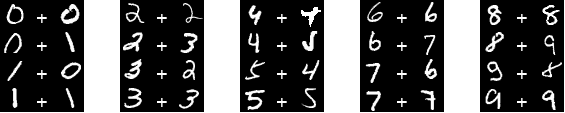
\includegraphics[max width=\textwidth]{dataset-examples}
	\caption{Some of the combinations of operands used for the experiment. Each combination shows only one sample selected from the MNIST dataset.}
	\label{fig:dataset-examples}
\end{figure}

A 5-fold cross-validation (discussed in Section \ref{sec:background-artificial-neural-networks-feed-forward-neural-networks}) approach is used to break down the dataset into a training, validation and test set such that for each combination of digits, six samples are used for training, two samples for validation and another two for testing. Since $k$ is set to 5, the training and testing of each of the five models is repeated five times, where the training, validation and testing samples for each combination are shuffled. The models for this experiment are exposed to all possible combinations of single digit operands during training. Some of the later experiments will only use a subset of the combinations for training and the rest for testing. After repeating the experiment five times for each model and recording the accuracies obtained from testing with the test sets, the mean accuracy and standard deviation for each model are calculated and used to compare the experiments graphically. A Hypothesis t-Test is also used to check the statistical difference of the means.

All networks trained have the same architecture, varying only in terms of the number of inputs. The architecture consists of two hidden LSTM layers, 512 units each, fully connected to an output layer, 20 units in length, composed of two one-hot vectors. This architecture was the result of trial and error and was found to have sufficient representation for the most difficult task at no detriment to the other tasks. The networks are trained using the Adam optimizer with the mean square error as the loss function and a learning rate of 0.001. Training is performed over 200 epochs (found to be sufficient for all methods) in batches of 100 and the set of weights performing best on the validation set is saved.  When evaluating the models, only noisy handwritten images are input and no symbol images are provided. The following paragraphs describe the five different architectures and training sets used.

\begin{figure}[t]
	\centering
	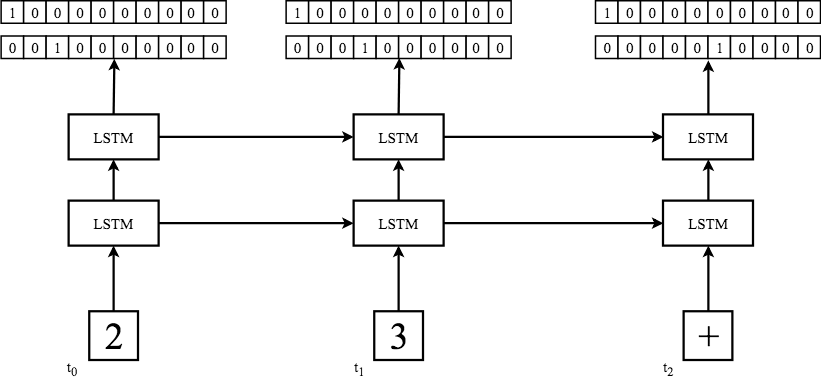
\includegraphics[max width=\textwidth]{sequential-model-symbols-only}
	\caption{Symbols Only (SO). A deep LSTM network that accepts a sequence of two operands and an operator. The operands are provided as the consistent symbol digits.}
	\label{fig:sequential-model-symbols-only}
\end{figure}

\paragraph{Symbols Only (SO).} The model learns to perform classification and addition using only the standard symbols (see Figure \ref{fig:sequential-model-symbols-only}). The input is a sequence of three 28x28 images, that are fed to the network one after the other. The first two images are that of the digits rendered clearly using a standard font. The third image is the plus operator. At each of the first two time steps the model is trained to classify the incoming digits producing two one-hot vectors representing the least and most significant digits of the input. Typically, the most significant digit will always be zero on these two time steps since we only use single digit inputs. When the plus sign is provided on the third time step, the network performs the addition operation, producing the result at the two one-hot vectors. The goal of training this model is to show that it is quite easy to do so using clear and consistent symbols.

\begin{figure}[t]
	\centering
	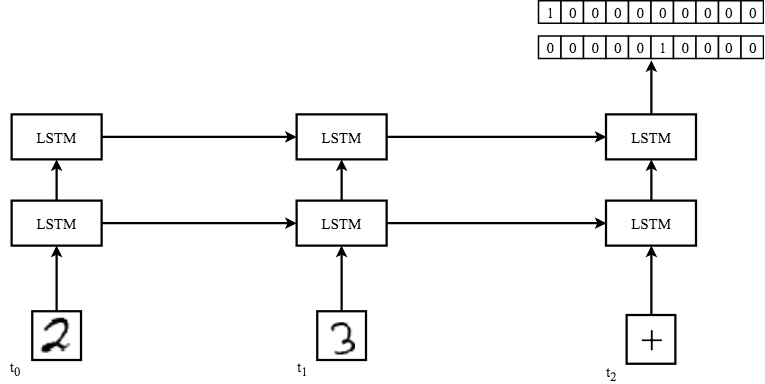
\includegraphics[max width=\textwidth]{sequential-model-noisy-only}
	\caption{Noisy Inputs Only (NO). A deep LSTM network that accepts a sequence of two operands and an operator. Only noisy operands are provided.}
	\label{fig:sequential-model-noisy-only}
\end{figure}

\paragraph{Noisy Inputs Only (NO).} The model learns to perform the addition using noisy handwritten digits without having to output the proper classes in the intermediate stages of the recurrent network (see Figure \ref{fig:sequential-model-noisy-only}). The input is a sequence of three 28x28 images, that are fed to the network one after the other. The first two images are that of noisy handwritten digit operands. The third image is the plus operator rendered in a standard font.  The goal of training the model using this method is to investigate the effectiveness of a network that is trained without the presence of symbols.

\begin{figure}[t]
	\centering
	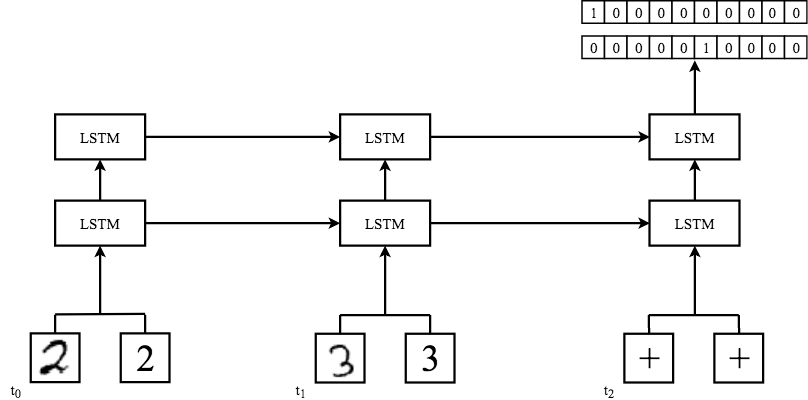
\includegraphics[max width=\textwidth]{sequential-model-symbols-noisy}
	\caption{Noisy and Symbol Inputs (NS). A deep LSTM network that accepts a sequence of two operands and an operator. Both the noisy operands and their corresponding symbolic information are provided alongside one another.}
	\label{fig:sequential-model-symbols-noisy}
\end{figure}

\paragraph{Noisy and Symbol Inputs (NS).} This model learns to perform addition without having to output the proper classes in the intermediate stages of the recurrent network (see Figure \ref{fig:sequential-model-symbols-noisy}). The input is a sequence of three pairs of 28x28 images, that are fed to the network one after the other. The first pair of images are of the first noisy handwritten digit operand and its matching standard symbolic digit. The second pair of images are for the second digit operand. The third pair of images are both the standard plus operator. The goal is to investigate the effect of introducing the clear symbol channel as an input (the explicit symbol) on the accuracy of the network.

\begin{figure}[t]
	\centering
	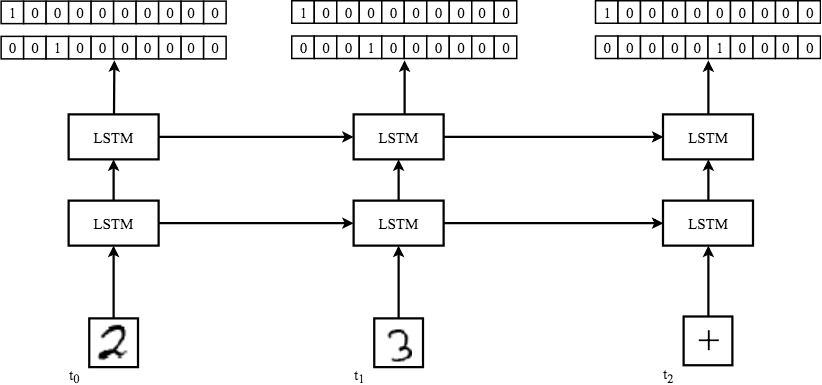
\includegraphics[max width=\textwidth]{sequential-model-noisy-classification}
	\caption{Noisy Inputs Only with Intermediate Classification (NC). A deep LSTM network that accepts a sequence of two operands and an operator. Noisy digits are provided as inputs and the network is trained to output the classes of each digit before performing the operation.}
	\label{fig:sequential-model-noisy-classification}
\end{figure}

\paragraph{Noisy Inputs Only with Intermediate Classification (NC).} The model learns to perform classification and addition on noisy digits only(see Figure \ref{fig:sequential-model-noisy-classification}). The input is a sequence of three 28x28 images, that are fed to the network one after the other. The first two images are that of handwritten digit operands. The third image is the plus operator. The model is trained to classify each incoming digit on each of the first two time steps by providing the class (as a one-hot vector) on the output during training and then perform the operation on the third time step. The goal is to investigate the effect of symbols on the accuracy of the network. However instead of using explicit symbols as inputs, the symbol is embedded in the LSTM context. By providing the classes of the handwritten digits while training, we believe that the network learns the symbolic information implicitly in the recurrent weights and then uses this information to aid in performing the mathematical operation.

\begin{figure}[t]
	\centering
	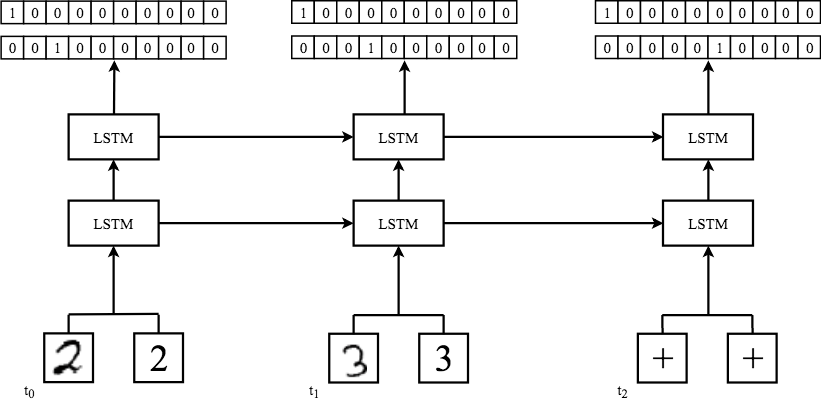
\includegraphics[max width=\textwidth]{sequential-model-noisy-symbol-classification}
	\caption{Noisy and Symbol Inputs with Intermediate Classification (NX). A deep LSTM network that accepts a sequence of two operands and an operator. Both the explicit and implicit symbols are provided.}
	\label{fig:sequential-model-noisy-symbol-classification}
\end{figure}

\paragraph{Noisy and Symbol Inputs with Intermediate Classification (NX).} This last model combines both methods of training used in NS and NC where the input includes the clear symbolic channel and the input classes are also provided on the output channel during training (see Figure \ref{fig:sequential-model-noisy-symbol-classification}). Here we investigate if a combination of the two methods of symbolic input improves on the individual approaches of the previous two methods.

\bigskip

While testing the trained Symbols Only (SO) model, we also test how well that model performs when tested on noisy handwritten digit inputs. We call this testing attempt \textbf{Symbols Tested with Noisy Inputs (SN)}. The objective is to see if training a recurrent neural network using only the idealized symbols will help the resulting model filter out the noise seen in the handwritten digits.

\subsubsection{Results}

\begin{table}[p!]
	\center
	\caption{A comparison of the mean accuracy and standard deviation of the models developed by the five methods. Also shown is the p-value of a hypothesis t-Test when compared to the NO method.}
	\label{tab:experiment-1-results-table}
	\begin{tabular}{ |c|c|c|c| } 
		\hline
		Method & Accuracy (\%) & Standard Deviation  & p-value, t-Test with NO Method\\ 
		SO & 100 & 0 & NA\\ 
		SN & 32.73 & 6.9 & NA\\
		NO & 60.16 & 4.5 & NA \\ 
		NS & 82.63 & 3.7 & 0.00317\\ 
		NC & 84.20 & 2.1 & 0.00102\\ 
		NX & 85.20 & 2.7 & 0.00043\\ 
		\hline
	\end{tabular}
\end{table}

\begin{figure}[p!]
	\centering
	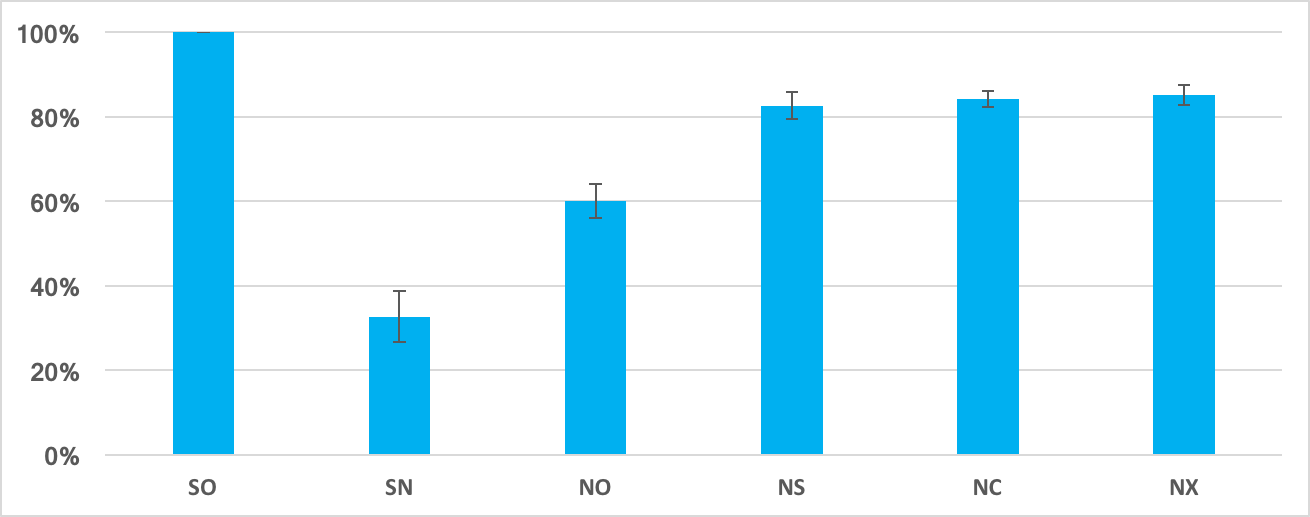
\includegraphics[max width=\textwidth]{experiment-1-results-chart}
	\caption{A comparison of the mean accuracy and 95\% confidence intervals of the models developed by the five methods.}
	\label{fig:experiment-1-results-chart}
\end{figure}

Table \ref{tab:experiment-1-results-table} and Figure \ref{fig:experiment-1-results-chart} compare the scores obtained from evaluating the models after training using the five methods. Training with symbols only (SO) produces the best model given the clear and consistent symbolic images. Training with the noisy handwritten digits only (NO) produces the worst model given the limited number of examples in the dataset. The three methods (NS, NC, NX) that developed models using noisy handwritten images as well as symbolic information show significant improvement over noisy only training. The results also show that there are no significant differences between the two methods of supplying symbols to the networks. However, the models that were trained using intermediate classification (NC and NX) have a smaller standard deviation.

\subsubsection{Discussion}

The experiments show that training a model with symbols results in a significant increase in the network accuracy over the models trained without the presence of symbols. The NC method that developed models to classify the operands as well as compute the addition did particularly well without the need for any additional inputs. The model does not accept a symbolic channel. Instead, by providing proper classification of the input operands while training, the model can be said to develop an implicit symbolic representation of the operands in the LSTM's recurrent context and transfer them from one step to the next.

The results presented in Table \ref{tab:experiment-1-results-table} and Figure \ref{fig:experiment-1-results-chart} show that there is no significant difference in the accuracy of the models trained using implicit symbols (NC) over the models trained with explicit symbols (NS). However, the experiment shows that the implicit symbol (NC) technique provides symbols to the network with the lowest predictive variance and therefore, we will use the implicit symbol technique in subsequent experiments.

Table \ref{tab:experiment-1-results-table} and Figure \ref{fig:experiment-1-results-chart} also show the results of testing the symbols only model (SO) using noisy data (SN). It is clear from the results that the network performs poorly. The model is not able to correctly map from the noisy handwritten digits to the classification labels and therefore is not able to successfully perform the addition.

\subsection{Experiment 2: Expanding Experiment 1 to use all four arithmetic operations} \label{sec:experiment-2}

\subsubsection{Objective}

The goal of this experiment is similar to Experiment 1 where we attempted to verify that the presence of symbols while training an artificial neural network results in significant increases in the network accuracy. Experiment 1 used only the addition operation. This experiment expands the dataset used to include all four arithmetic operations.

\subsubsection{Method}

For this experiment we use the \textbf{Noisy Inputs with Intermediate Classification (NC)} from the previous experiment as the model that is trained in the presence of symbols. Figure \ref{fig:sequential-model-symbols-noisy-times} depicts the NC model learning to do multiplication. \textbf{The Noisy Inputs Only (NO)} model is also used for comparison as the model trained without symbols. NO is slightly modified to provide output on its intermediate time steps. The output provided during training for these intermediate time steps is a vector with all its features set to a dummy value of 0.5 to signify that no symbol is provided. Figure \ref{fig:sequential-model-noisy-only-divide} shows an example of the NO model performing division.

The dataset used for Experiment 1 is expanded to include four different arithmetic operations (addition, subtraction, multiplication and division). For each operation, single digit inputs from the range of 0 to 9 are used to form combinations of operands and for each combination, ten MNIST examples are sampled. For both addition and multiplication, all 100 combinations are included in the dataset. However, for subtraction and division the combinations are selected so that for subtraction, no combinations that would result in negative outputs would be included and for division, division by zero is avoided. K-fold cross-validation is used, with k set to 5, to split the samples of each combination into a training, validation and test set. The training and testing of each model is repeated five times and the accuracy obtained on the test set is recorded for each attempt. Just like in Experiment 1, all combinations of digits are provided for training.

\begin{figure}[t]
	\centering
	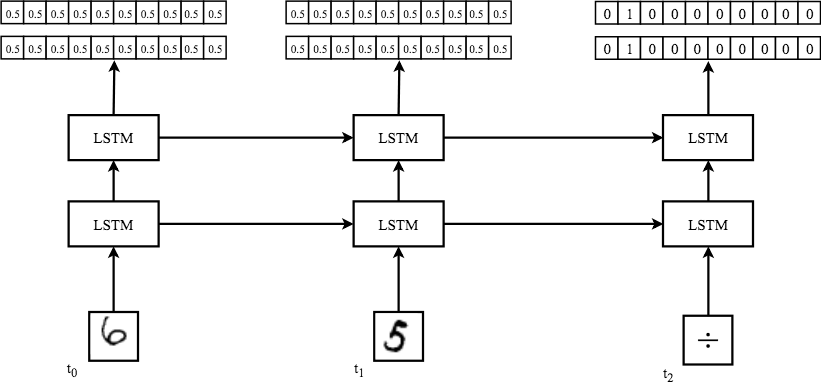
\includegraphics[max width=\textwidth]{sequential-model-noisy-only-divide}
	\caption{The Noisy Inputs Only (NO). A deep LSTM network that accepts a sequence of two operands and an operator modeling the operation: 6 / 5. Only noisy operands are provided. The output represents the quotient and the remainder, which are both 1.}
	\label{fig:sequential-model-noisy-only-divide}
\end{figure}

Both models have the same architectures used in Experiment 1. The models accept a sequence of three 28x28 images. The first two images are of the handwritten digits representing the operands of the operation. The third image is that of the operator. The models output two one-hot vectors representing the least and most significant values of the output at each time step. When each of the operands is presented, the network attempts to output the correct signals on the one-hot vector outputs representing the value of the digit presented on the input. When finally the operator is presented, the network is trained to perform the operation and output the result. Both models use two hidden LSTM layers each with 512 units.

\begin{figure}[t]
	\centering
	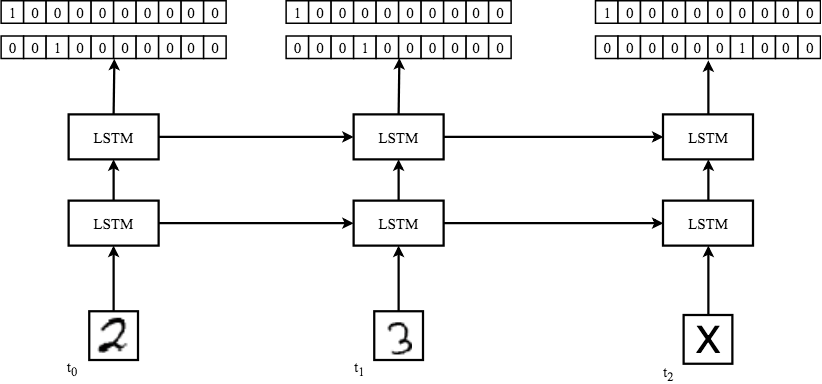
\includegraphics[max width=\textwidth]{sequential-model-symbols-noisy-times}
	\caption{Noisy Inputs with Intermediate Classification (NC). A deep LSTM network that accepts a sequence of two operands and an operator modeling the operation 2 x 3. Both the noisy operands and their corresponding symbolic information are provided alongside one another.}
	\label{fig:sequential-model-symbols-noisy-times}
\end{figure}

\subsubsection{Results}

\begin{table}[p]
	\center
	\caption{A comparison of the mean accuracy and standard deviation of the models trained with and without classification on all four arithmetic operations. Also shown is the p-value of a hypothesis t-Test when compared to the NO method.}
	\label{tab:experiment-2-results-table}
	\begin{tabular}{ |c|c|c|c| } 
		\hline
		Method & Accuracy (\%) & Standard Deviation  & p-value, t-Test with NO Method\\ 
		NO & 60.75 & 0.02 & NA \\  
		NC & 77.36 & 0.03 & 0.00092\\  
		\hline
	\end{tabular}
\end{table}

\begin{figure}[p]
	\centering
	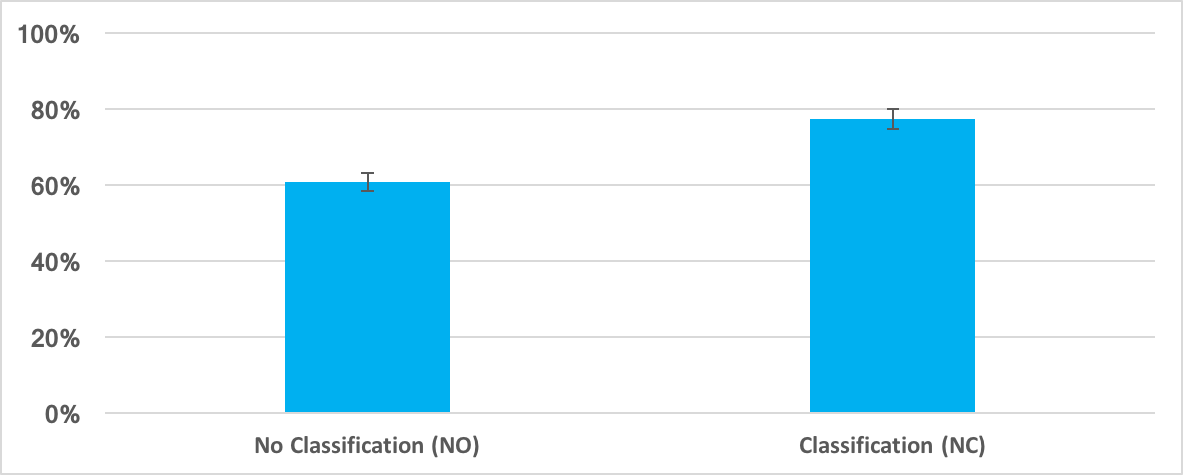
\includegraphics[max width=\textwidth]{experiment-2-results-chart}
	\caption{A comparison of the mean accuracy and 95\% confidence intervals of the models trained with and without classification on all four arithmetic operations.}
	\label{fig:experiment-2-results-chart}
\end{figure}

\begin{table}
	\center
	\caption{The mean accuracies of each arithmetic operation when tested on both the NO and NC models.}
	\label{tab:experiment-2-operations-table}
	\begin{tabular}{ |c|c|c|c|c| } 
		\hline
		Method & Addition (\%) & Subtraction (\%)  & Multiplication (\%) & Division (\%)\\ 
		NO & 63.35 & 60.77 & 61.4 & 57.48\\  
		NC & 78.5 & 77.71 & 80.23 & 73.0\\  
		\hline
	\end{tabular}
\end{table}

\begin{figure}[t]
	\centering
	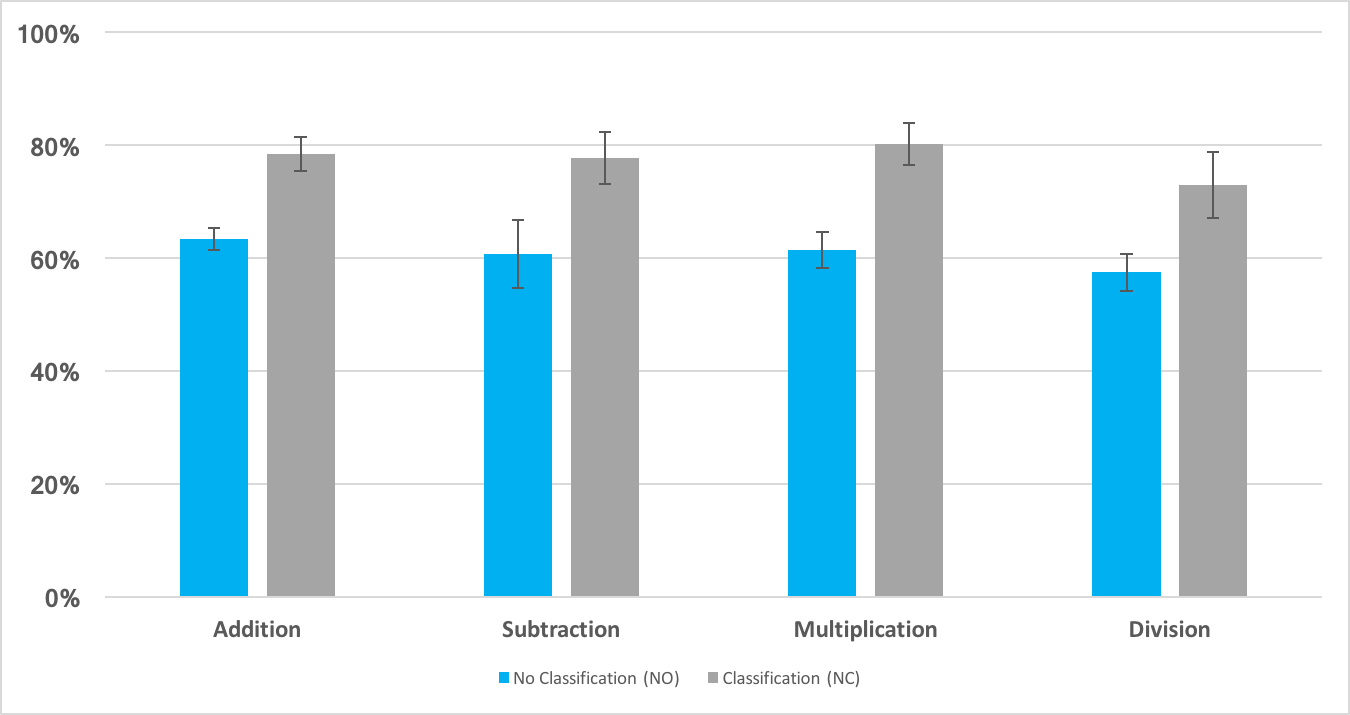
\includegraphics[max width=\textwidth]{experiment-2-operations-chart}
	\caption{A comparison of the mean accuracy and 95\% confidence intervals of each arithmetic operation on both models trained with and without classification.}
	\label{fig:experiment-2-operations-chart}
\end{figure}

Table \ref{tab:experiment-2-results-table} and Figure \ref{fig:experiment-2-results-chart} compare the results of the model trained without symbols (NO) with the model trained with symbols (NC). The model trained in the presence of symbols performs significantly better than the one trained without symbols. Table \ref{tab:experiment-2-operations-table} and Figure \ref{fig:experiment-2-operations-chart} show the accuracies obtained using each of these models when tested on each arithmetic operator independently.

\subsubsection{Discussion}

This experiment shows that the LSTM recurrent neural networks are capable of learning various types of arithmetic operations on images of handwritten digits and that the presence of symbolic knowledge during training significantly improves the accuracy of these models. With the exception of division, Table \ref{tab:experiment-2-operations-table} and Figure \ref{fig:experiment-2-operations-chart} show that when analyzing the accuracies of the models on each operator independently, we see that the mean accuracies are close to one another and close to the overall mean accuracy of the models. Division is a more complicated operation that involves finding a quotient and a remainder which could account of the reduced performance.

\subsection{Experiment 3: Comparing the Effect of Varying the Presence of Symbols on the Accuracy of Training} \label{sec:experiment-3}

\subsubsection{Objective}

In the previous experiments, we showed that the presence of symbols improves the effectiveness of recurrent neural networks in learning to perform arithmetic on images of handwritten digits when training using an impoverished dataset. In Section \ref{sec:theory-hypothesis-multi-task-learning} we proposed that this would be the expected behavior due to the beneficial effect of multi-task learning on all tasks being learned by the recurrent networks. In this experiment we attempt to further demonstrate this benefit.
 
Our goal is to show the relationship between the accuracy of the model in classifying the inputs on the intermediate time steps and the accuracy of the same model in producing the correct output for the given mathematical operation. The existence of this relationship should indicate that by correctly classifying the digits, the recurrent neural network is able to create internal features on the first two time steps that are then used on the third time step to perform the arithmetic operation. In the absence of these clear features, the network would rely only on the noisy handwritten inputs.

Besides establishing the relationship between the classification accuracy and the mathematical accuracy of our models, we also to vary the percentage of symbols included with each training example. The expected outcome here is that the higher the percentage of symbols present, the more accurate the classification accuracy will be and in turn the higher the accuracy of performing the arithmetic operation.

\subsubsection{Method}

The architectures constructed for this experiment are the same as the ones used in the previous two experiments. The models accept a sequence of three 28x28 images. The first two images are of the handwritten digits representing the operands of the operation. The third image is that of the operator. The networks output two one-hot vectors. When each of the operands are presented, the model attempts to output a one-hot encoded vector of the value of the operand. When the operator is presented, the network learns to compute and present the output. Two hidden layers are used each containing 512 LSTM units. All four arithmetic operations are used together during training.

The dataset used in Experiment 2 in Section \ref{sec:experiment-2} is replicated into five sets, with some modifications, for use in this experiment. Each combination now includes eight MNIST samples instead of ten, where four are used for training, two for validation and two for testing. This makes the process of varying symbols easier. Each of the five replicas are modified to vary the number of symbols included with each digit combination during training. The first set has no symbols, meaning a vector with all features set to 0.5 is provided as a dummy output for the intermediate classification time steps. The second dataset has 25\% of the MNIST samples in each combination include a symbol whereas the rest use the 0.5 dummy values. The 25\% symbols are distributed such that, out of the four training samples, one has a symbol and the rest do not. The third dataset has 50\% symbols meaning that out of the four training examples per combination two include their corresponding symbols. The fourth dataset has 75\% of the training examples include symbols, meaning three out of four examples per combination include their corresponding symbol. Finally, the fifth dataset, the 100\% symbols dataset, includes symbols for all examples.

Five models were trained each using one of the datasets described above. The networks were trained using the Adam optimizer with the mean square error as the loss function and a learning rate of 0.001. Training is performed over 200 epochs in batches of 100 and the model performing best on the validation set is saved. Each model is trained five times using 5-fold cross-validation where all digit combinations are used. Instead of recording the accuracy of each model as was done in the previous experiments, here we split the accuracy into four new metrics. They are as follows:
\begin{itemize}
	\item False Classification/False Operation \textbf{(FC/FO)}: The percentage of test samples that classify incorrectly during the intermediate time steps that also produce incorrect outputs for the mathematical operation.
	\item False Classification/True Operation \textbf{(FC/TO)}: The percentage of test samples that classify incorrectly during the intermediate time steps that produce correct outputs for the operation.
	\item True Classification/False Operation \textbf{(TC/FO)}: The percentage of test samples that classify correctly during the intermediate time steps that produce incorrect outputs for the operation.
	\item True Classification/True Operation \textbf{(TC/TO)}: The percentage of test samples that classify correctly during the intermediate time steps that also produce correct outputs for the operation.
\end{itemize}

The epoch number that results in the most optimum set of weights for each percentage of symbols used is also recorded, to understand the effect of symbols on the efficiency of training with and without symbols.

\subsubsection{Results}

\begin{table}[p]
	\center
	\caption{A comparison of the mean FC/FO percentage, standard deviation and the p-value of a hypothesis t-Test when compared to the 0\% symbols model.}
	\label{tab:experiment-3-results-table-fcfo}
	\begin{tabular}{ |c|c|c|c| } 
		\hline
		\% Symbols Present & FC/FO (\%) & Standard Deviation  & p-value\\ 
		0\% & 55.8 & 0.063 & NA \\  
		25\% & 39.80 & 0.03 & 0.00493\\  
		50\% & 26.20 & 0.042 & 0.00141 \\  
		75\% & 17.05 & 0.023 & 0.00033\\  
		100\% & 13.60 & 0.012 & 0.00016\\  
		\hline
	\end{tabular}
\end{table}

\begin{table}[p]
	\center
	\caption{A comparison of the mean FC/TO percentage, standard deviation and the p-value of a hypothesis t-Test when compared to the 0\% symbols model.}
	\label{tab:experiment-3-results-table-fcto}
	\begin{tabular}{ |c|c|c|c| } 
		\hline
		\% Symbols Present & FC/TO (\%) & Standard Deviation  & p-value\\ 
		0\% & 37.55 & 0.0672 & NA \\  
		25\% & 27.95 & 0.0387 & 0.0031\\  
		50\% & 11.50 & 0.0351 & 0.00141 \\  
		75\% & 5.40 & 0.0137 & 0.00084\\  
		100\% & 2.45 & 0.0042 & 0.00016\\  
		\hline
	\end{tabular}
\end{table}

\begin{table}[p]
	\center
	\caption{A comparison of the mean TC/FO percentage, standard deviation and the p-value of a hypothesis t-Test when compared to the 0\% symbols model.}
	\label{tab:experiment-3-results-table-tcfo}
	\begin{tabular}{ |c|c|c|c| } 
		\hline
		\% Symbols Present & TC/FO (\%) & Standard Deviation  & p-value\\ 
		0\% & 3.70 & 0.0106 & NA \\  
		25\% & 15.05 & 0.0214 & 0.00183\\  
		50\% & 23.20 & 0.01024 & 0.02209 \\  
		75\% & 13.55 & 0.0107 & 0.00013\\  
		100\% & 8.15 & 0.0158 & 0.01742\\  
		\hline
	\end{tabular}
\end{table}

\begin{table}[p]
	\center
	\caption{A comparison of the mean TC/TO percentage, standard deviation and the p-value of a hypothesis t-Test when compared to the 0\% symbols model.}
	\label{tab:experiment-3-results-table-tcto}
	\begin{tabular}{ |c|c|c|c| } 
		\hline
		\% Symbols Present & TC/TO (\%) & Standard Deviation  & p-value\\ 
		0\% & 2.95 & 0.0166 & NA \\  
		25\% & 17.20 & 0.0148 & 0.00043\\  
		50\% & 39.10 & 0.0853 & 0.00179 \\  
		75\% & 64.00 & 0.0301 & 0.0\\  
		100\% & 75.80 & 0.0213 & 0.0\\  
		\hline
	\end{tabular}
\end{table}

\begin{figure}[p]%
	\centering
	\subfloat[False Classification/False Operation]{{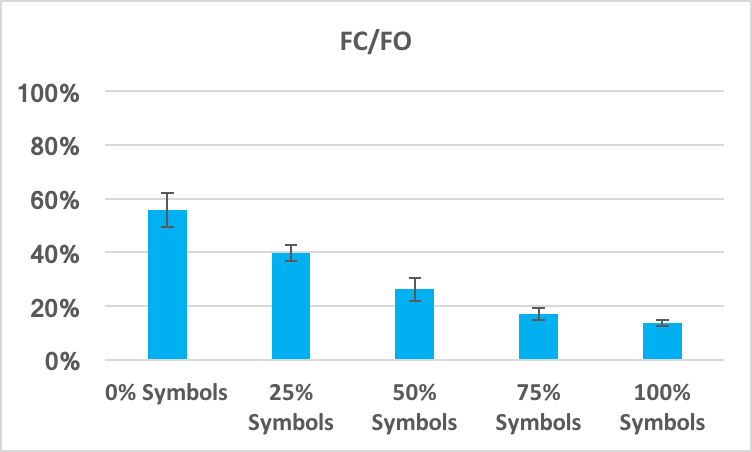
\includegraphics[width=0.5\textwidth]{experiment-3-results-chart-fc-fo} }}\label{fig:experiment-3-results-chart-fc-fo}%
	\subfloat[False Classification/True Operation]{{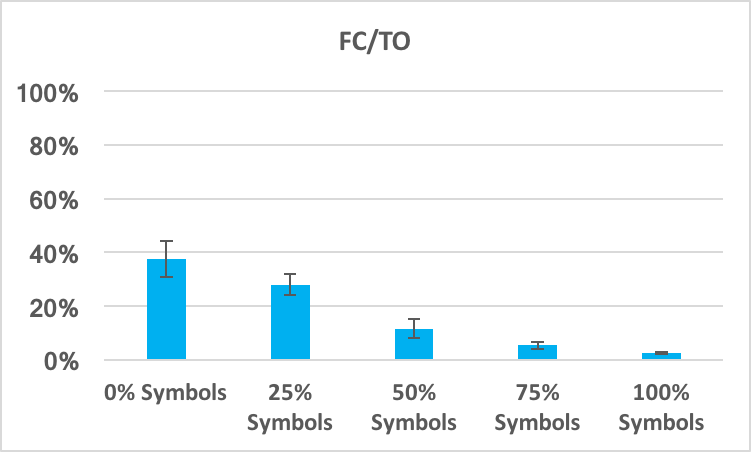
\includegraphics[width=0.5\textwidth]{experiment-3-results-chart-fc-to} }}\label{fig:experiment-3-results-chart-fc-to}%
	
	\subfloat[True Classification/False Operation]{{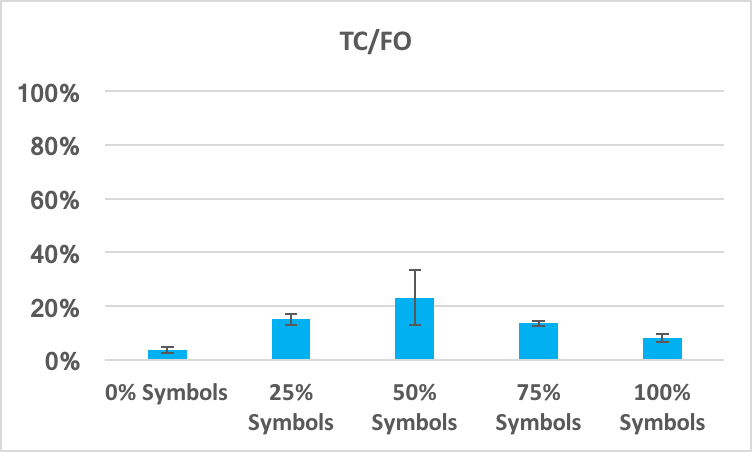
\includegraphics[width=0.5\textwidth]{experiment-3-results-chart-tc-fo} }}\label{fig:experiment-3-results-chart-tc-fo}%
	\subfloat[True Classification/True Operation]{{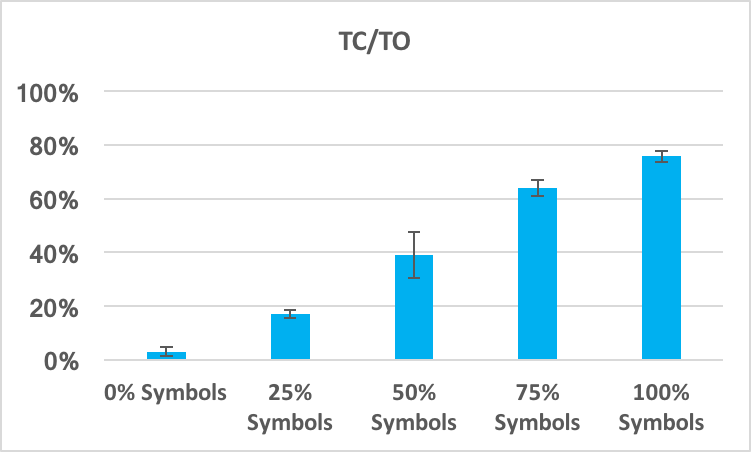
\includegraphics[width=0.5\textwidth]{experiment-3-results-chart-tc-to} }}\label{fig:experiment-3-results-chart-tc-to}%
	\caption{A comparison of the four metrics FC/FO, FC/TO, TC/FO, TC/TO along with their corresponding 95\% confidence intervals for each of the five models developed.}%
	\label{fig:experiment-3-results-chart}%
\end{figure}

Tables \ref{tab:experiment-3-results-table-fcfo} to \ref{tab:experiment-3-results-table-tcto} present the mean FC/FO, FC/TO, TC/FO, TC/TO accuracies for each of the datasets used along with the standard deviations and the p-test score of a hypothesis t-Test compared to the 0\% model. Figure \ref{fig:experiment-3-results-chart} shows the same results presented in graphical form. Table \ref{tab:experiment-3-results-epochs} presents the number of epochs needed for the network to discover the optimum set of weights for each of the five datasets.

\begin{table}[h]
	\center
	\caption{A comparison of the average epoch number at which the optimum weights were discovered for each of the models trained.}
	\label{tab:experiment-3-results-epochs}
	\begin{tabular}{ |c|c| } 
		\hline
		\% Symbols Present & Mean Epoch Number\\ 
		0\% Symbols & 4.2\\  
		25\% Symbols & 10.0\\  
		50\% Symbols & 11.0\\  
		75\% Symbols & 15.8\\  
		100\% Symbols & 38.0\\  
		\hline
	\end{tabular}
\end{table}

\subsubsection{Discussion}

It is clear from Table \ref{tab:experiment-3-results-table-tcto} and Figure \ref{fig:experiment-3-results-chart}(d) that more training examples with symbolic classification data improves the correct output of the operations (TO), particularly when the classification is also correct (TC) (75.8\% of the time with 100\% symbols), and rarely, as shown in Table \ref{tab:experiment-3-results-table-fcto} and Figure \ref{fig:experiment-3-results-chart}(b) when the classification is incorrect (FC) (only 2.45\% of the time with 100\% symbols).

Inversely, as shown in Table \ref{tab:experiment-3-results-table-fcfo} and Figure \ref{fig:experiment-3-results-chart}(a), incorrect output (FO) for a mathematical operator occurs frequently with false classification (FC) (13.6\% of the time with 100\% symbols). It also makes sense that as the percentage of false classifications (FC) declines (due to more symbols in the training set) the percentage of false operation (FO) outputs also declines, because the probability of an operation being performed on the wrong operands decreases.

These results show that the presence of symbols improves the accuracy of classification which in turn improves the accuracy of performing the operation. Classifying the handwritten operands creates an internal representation of the digits that is retained by the LSTM recurrent connections. In the presence of symbols, this representation is learned more consistently for each digit, reducing the variations of the handwritten digits and therefore improving the model's accuracy when performing the operation. This is a recurrent multi-task learning effect that provides beneficial results.

The TC/FO graph of Figure \ref{fig:experiment-3-results-chart}(c) on the other hand says that incorrect operation output (FO) occurs most frequently (23.2\% of the time) when 50\% of the training examples have classification signals and the test examples operands are classified correctly (TC). In fact, the percentage of FO examples is almost as high for TC/FO at 50\%, 75\% and 100\% as they are for FC/FO. This makes it clear that there are limits to the system's ability to get correct operation outputs (TO) even when it has TC for certain examples.

\begin{figure}[t]
	\centering
	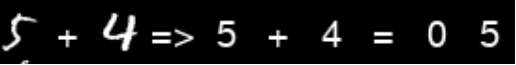
\includegraphics[max width=\textwidth]{tc-fo-example}
	\caption{Example of a TC/FO operation. The operation 5 + 4 is classified correctly, however the output is still false.}
	\label{fig:tc-fo-example}
\end{figure}

This limitation can be due to the fact that the noisy handwritten digits still retain some influence over the network that forces the model to use the noisy inputs for pattern matching instead of the clearer internal representations. Figure \ref{fig:tc-fo-example} shows an example of one of the TC/FO cases trained with 50\% symbols. The handwritten digits are shown along with the result of classification and the result of the operation. The operation is that of 5 + 4. The handwritten digits are classified correctly, however the output of 5 is incorrect. This example shows that the model was still being influenced by the confusing handwritten digits. It might have confused the first operand 5 for the digit 1.

Looking at the results in Table \ref{tab:experiment-3-results-epochs} we see that the more symbols are used the longer it takes for the network to converge onto an optimum decision function. We initially predicted that providing clearer symbols would make the learning process more efficient, but that apparently is not the case. We now understand that without the symbolic information, the gradient descent algorithm will converge to a local minimum early in the training process resulting in the poor classification results and therefore less accurate mathematical operation output. The introduction of more symbols forces the gradient descent algorithm to search longer for an appropriate representation in weight space that is compatible with both the symbol classification and the mathematical operation output.
